\documentclass[12pt]{article}
\usepackage[margin=1.5cm]{geometry}
\usepackage{parskip}
\usepackage{amsmath}
\usepackage{amssymb}
\usepackage{amsfonts}
\usepackage{enumitem}
\usepackage{graphicx}
\usepackage{stmaryrd}
\graphicspath{ {./images/} }


\begin{document}
\begin{enumerate}[label=(\alph*)]

  \item
    In an LTL formula, to reason about all reachable states, our formula has to be of the form $G (\phi)$, which can be interpreted as: for every path $\pi$ from every reachable state $s$, $\phi$ holds in $\pi$.

    So, we need a $\phi$ that is interpreted as: if $p$ is true at a state, then there exists a path from that state such that $q$ is true at the next state in that path.

    Consider the following two models:

    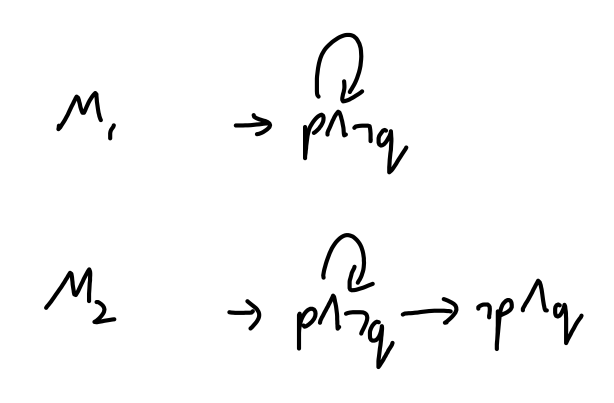
\includegraphics[scale=0.3]{simulation}

    Here, $M_2$ is a simulation of $M_1$, since the initial states and labels match in $M_2$, and every path in $M_1$ has a corresponding path in $M_2$.

    Suppose such a $\phi$ did exist. Clearly $\phi$ is true in $M_2$, and by simulation $\phi$ should be true in $M_1$, but it is not true in $M_1$, and thus no such $\phi$ can exist.

    \item
      Such a formula does exist:

      $AG (p \implies E (X q))$
        
    \end{enumerate}
\end{document}
